\chapter{Анализ технологического процесса 3D-печати и причин возникновения дефектов}

\section{Технология послойного наплавления: принципы, ограничения и критичные параметры процесса}

В данной работе рассматривается технология печати методом послойного наплавления, для которой разрабатывается контур мониторинга и раннего обнаружения отклонений. Метод послойного наплавления (Fused Deposition Modeling, FDM)~-- аддитивный метод, при котором полимерная нить подается в нагревательный блок, расплавляется и через сопло наносится слоями, формируя геометрию изделия~\cite{лысыч2014области}.

Схема устройства FDM-принтера приведена на рисунке~\ref{fig:FDM}.

\begin{figure}[h!]
\centering
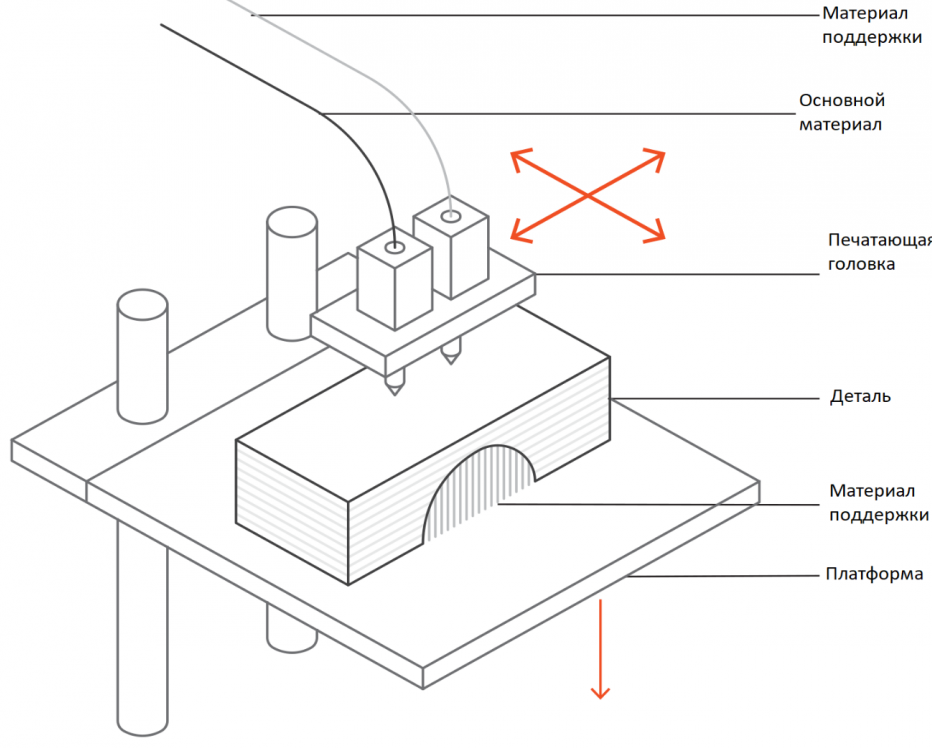
\includegraphics[width=0.75\hsize]{fig/FDM.png}
\caption{Схема устройства FDM-принтера}
\label{fig:FDM}
\end{figure}

Технологический цикл метода включает подготовку модели, формирование управляющей траектории и последовательное построение изделия слоями. Качество результата в таком процессе определяется не одним параметром, а совокупностью факторов, связанных с материалом, состоянием оборудования, условиями среды и корректностью цифровой подготовки задания.

С практической точки зрения дефекты FDM-печати целесообразно рассматривать как следствие нарушения устойчивости процесса. Если в одном из звеньев технологической цепочки возникает отклонение, оно переносится на последующие слои и может усиливаться по мере роста изделия. Поэтому анализ причин дефектов должен выполняться комплексно, а не только через локальные корректировки отдельных настроек.

Важным элементом процесса является филамент -- полимерный расходный материал в виде непрерывной нити, который подается в экструдер, расплавляется и формирует дорожки слоя. Свойства филамента непосредственно влияют на стабильность экструзии, характер межслойного сцепления и повторяемость геометрии. Даже при исправной механике принтера нестабильное качество материала способно привести к систематическим отклонениям результата.

Среди типовых источников проблем со стороны материала выделяются неоднородность состава, отклонения диаметра нити, повышенная влажность и наличие посторонних включений. Неоднородность расплава вызывает неравномерную подачу, что отражается на форме дорожек и точности контуров. Влажный материал при нагреве может давать нестабильную экструзию и ухудшать качество поверхности, а твердые включения повышают риск частичных засоров и ускоренного износа сопла.

На итог печати влияет не только химический состав филамента, но и его физическое состояние в момент использования. Перегибы нити, повышенное трение в тракте подачи и нестабильная намотка катушки создают дополнительные возмущения потока материала. В результате возникают локальные нарушения структуры слоя, которые визуально проявляются как ухудшение геометрии, неоднородность поверхности и снижение эксплуатационной пригодности детали.

Отдельную группу причин образуют факторы оборудования и кинематики: люфты, износ механических узлов, нестабильность перемещений, загрязнение рабочих элементов и недостаточная повторяемость позиционирования. Эти отклонения не всегда приводят к мгновенному браку, однако постепенно формируют накопительный эффект, при котором небольшие погрешности первых слоев переходят в заметные дефекты на более поздних стадиях печати.

Существенное влияние оказывают и внешние условия выполнения задания. Колебания температуры, локальные потоки воздуха и нестабильность теплообмена в рабочей зоне изменяют режим формирования слоя и межслойного контакта. Для длительных заданий это особенно критично, поскольку продолжительность процесса повышает чувствительность к малым, но систематическим воздействиям среды.

Причины дефектов в FDM-печати удобно группировать по четырем блокам: материал, оборудование, цифровая подготовка и внешние условия. Такая структура позволяет связать наблюдаемое отклонение с вероятным источником и выбрать корректирующее действие на уровне причины, а не только на уровне внешнего симптома. Для задач автоматизированного контроля это принципиально, так как повышает достоверность диагностики и снижает риск повторения дефекта в следующих циклах печати.

Таким образом, филамент следует рассматривать как один из ключевых факторов устойчивости FDM-процесса наряду с состоянием принтера и условиями эксплуатации. Комплексный учет этих факторов формирует основу для раннего обнаружения отклонений и для построения системы, способной своевременно реагировать на признаки ухудшения качества печати. Далее рассматриваются основные классы дефектов FDM-печати.

\section{Классы дефектов печати и факторы их возникновения в реальных условиях эксплуатации}

В реальных условиях эксплуатации дефекты FDM-печати формируются не как изолированные события, а как результат совокупного влияния материала, оборудования, подготовленного задания и внешней среды. Для практической задачи мониторинга важно перечислить возможные отклонения. Отдельно необходимо выделить классы, которые одновременно являются критичными для процесса и устойчиво наблюдаются по визуальным признакам во время печати.

С инженерной точки зрения дефекты целесообразно разделять по последствиям: ухудшение геометрии и внешнего вида изделия, снижение прочности, срыв текущего задания и риск повреждения узлов принтера. Для разработки системы автоматического обнаружения приоритет получают состояния, при которых задержка реакции приводит к наибольшим потерям материала, времени и ресурса оборудования.

В данной работе рассматривается широкий набор возможных отклонений. В качестве целевых классов для автоматического распознавания выбраны четыре наиболее критичных дефекта: растрескивание, отлипание модели от стола, дефект типа «спагетти» и смещение слоев. Такой выбор позволяет сосредоточить обучение модели на сценариях с максимальным практическим эффектом от раннего обнаружения.

Растрескивание отражает нарушение целостности изделия и связано с потерей межслойной прочности. На практике этот дефект проявляется при неблагоприятном тепловом режиме, неравномерном охлаждении и недостаточной адгезии между слоями. Даже локальные трещины ухудшают эксплуатационные свойства детали и часто делают результат печати непригодным для целевого применения.

Отлипание модели от стола является критическим дефектом начальной стадии, поскольку нарушает базовую геометрию всего дальнейшего построения. Причинами обычно выступают нестабильная адгезия первого слоя, состояние рабочей поверхности и совокупность факторов, влияющих на удержание детали в процессе роста высоты. При развитии этого отклонения печать теряет воспроизводимость и переходит в аварийный режим.

Дефект типа «спагетти» возникает при потере корректного контакта экструдируемого материала с моделью, когда подача пластика продолжается, но формирование слоя уже нарушено. В результате материал накапливается в виде хаотичных нитей, а задание фактически выполняется вхолостую. Этот сценарий быстро увеличивает расход материала и машинного времени, а также затрудняет последующее восстановление рабочего состояния принтера.

Смещение слоев относится к дефектам, при которых траектория укладки материала сдвигается относительно ранее сформированной части изделия. Визуально это проявляется в виде ступенчатого смещения контуров и несоосности стенок, что приводит к искажению геометрии и снижению пригодности детали. Причинами смещения обычно являются пропуски шагов приводов, перегрузка кинематики, недостаточное натяжение ремней, заедания механики или столкновения с деформациями изделия; поэтому данный дефект рассматривается как приоритетный для раннего выявления и своевременного реагирования.

Важной особенностью реальной эксплуатации является динамика развития дефектов: например, отлипание может привести к «спагетти», а нарушения работы приводов и кинематики — к смещению слоев. Следовательно, система контроля должна учитывать динамику процесса и обнаруживать признаки отклонений на ранней стадии, до перехода в более тяжелый сценарий.

Таким образом, в рамках работы основное внимание сосредоточено на четырех целевых классах дефектов: растрескивание, отлипание, «спагетти» и смещение слоев. На этих группах формируется разметка данных и выполняется обучение нейросетевой модели обнаружения, поскольку именно они имеют наибольшее значение для устойчивости печати и безопасности эксплуатации оборудования.

Сводная характеристика приоритетных дефектов для раннего обнаружения приведена в таблице~\ref{table:defects_priority}.

\begin{table}[ht]
\caption{Сводная характеристика приоритетных дефектов для раннего обнаружения}
\label{table:defects_priority}
\scriptsize
\renewcommand{\arraystretch}{1.05}
\setlength{\tabcolsep}{3pt}
\centering
\begin{tabular}{|>{\raggedright\arraybackslash}m{70pt}|>{\raggedright\arraybackslash}m{86pt}|>{\raggedright\arraybackslash}m{88pt}|>{\raggedright\arraybackslash}m{58pt}|>{\raggedright\arraybackslash}m{86pt}|}
\hline
Дефект & Ранние визуальные признаки & Влияние на процесс & Приоритет реагирования & Базовое действие системы \tabularnewline
\hline
Растрескивание & Трещины, расхождение слоев, нарушение поверхности & Потеря прочности, риск непригодности детали & Высокий & Фиксация события, уведомление, контроль динамики \tabularnewline
\hline
Отлипание модели от стола & Смещение модели, потеря контакта первого слоя со столом & Срыв геометрии, потеря воспроизводимости печати & Критический & Немедленная пауза и остановка при подтверждении отклонения \tabularnewline
\hline
Дефект типа «спагетти» & Хаотичные нити пластика вне контура модели & Бесполезный расход материала, потеря машинного времени & Критический & Остановка задания, уведомление, подготовка к перезапуску \tabularnewline
\hline
Смещение слоев & Ступенчатый сдвиг контуров, несоосность слоев & Искажение геометрии, риск непригодности детали & Высокий & Фиксация события, уведомление, пауза при подтверждении отклонения \tabularnewline
\hline
\end{tabular}
\end{table}

Далее рассматривается влияние выделенных дефектов на качество изделий, расход материала и надежность оборудования.

\section{Влияние дефектов на качество изделий, расход материала и надежность оборудования}

Анализ последствий дефектов в процессе~3D-печати необходим для оценки устойчивости технологического цикла и эффективности эксплуатации оборудования. Если отклонения не выявляются на ранней стадии, они переходят из локальной проблемы качества в фактор, влияющий на весь производственный контур. В результате возрастает доля незавершенных заданий, снижается предсказуемость результата и увеличиваются совокупные издержки выполнения печати.

Первый уровень последствий связан с качеством готового изделия. Дефекты нарушают геометрию детали, равномерность структуры и целостность межслойных связей, из-за чего итоговый объект может не соответствовать требованиям по размерам и форме. Для прикладных задач это означает снижение повторяемости результата: даже при одинаковом задании итоговые характеристики деталей становятся нестабильными, что усложняет последующую сборку и использование изделий по назначению.

Второй уровень последствий проявляется в эксплуатационной пригодности изготовленной детали. При наличии дефектов снижается фактическая прочность изделия, ухудшается устойчивость к рабочим нагрузкам и повышается вероятность отказа в процессе применения. Даже если деталь сохраняет внешний вид, внутренние нарушения структуры могут ограничивать срок службы и требовать повторного изготовления, что снижает практическую ценность результата печати.

Третий уровень связан с расходом материалов и затратами машинного времени. Любое прерванное или некачественное задание приводит к прямым потерям филамента, а повторный запуск увеличивает длительность выполнения одной и той же технологической операции. При серийных задачах такие потери накапливаются, формируя дополнительную нагрузку на оператора и уменьшая фактическую производительность печатного контура.

Отдельно необходимо учитывать влияние дефектов на надежность оборудования. При работе в условиях отклонений возрастают механические и тепловые нагрузки на узлы подачи материала и печатающую головку, увеличивается частота обслуживающих операций и сокращаются интервалы стабильной работы без вмешательства. Это приводит к ускоренному износу отдельных компонентов, повышает вероятность внеплановой остановки и увеличивает трудоемкость восстановления рабочего состояния принтера.

Существенным последствием является рост простоев оборудования. Время, затрачиваемое на остановку задания, диагностику причин, очистку рабочей зоны, повторную подготовку поверхности и перезапуск печати, исключает принтер из полезного производственного цикла. При регулярном повторении таких сценариев снижается пропускная способность системы, а график выполнения заданий становится менее управляемым и менее прогнозируемым.

В совокупности дефекты выступают не только как показатель качества отдельной детали, но и как фактор технико-экономической эффективности всей системы~3D-печати. Их влияние одновременно затрагивает качество продукции, стабильность эксплуатации оборудования и себестоимость выполнения задач. Следовательно, оценка и раннее обнаружение отклонений должны рассматриваться как обязательный элемент управления процессом, а не как дополнительная операция контроля после завершения печати.

С учетом указанных последствий в рамках работы приоритет отдается четырем группам дефектов, оказывающим наибольшее влияние на устойчивость цикла и безопасность эксплуатации: растрескивание, отлипание модели от стола, дефект типа «спагетти» и смещение слоев. Концентрация обучения нейросетевой модели на этих группах повышает практическую значимость автоматического контроля. За счет такого фокуса система обеспечивает более полезный эффект от раннего реагирования.

\section{Методы мониторинга процесса печати и подходы к раннему обнаружению отклонений}

Мониторинг процесса~3D-печати является ключевым условием устойчивой работы производственного контура, поскольку отклонения формируются во времени и накапливаются от слоя к слою. Если признаки нарушения фиксируются поздно, система теряет возможность локального вмешательства и переходит к затратному сценарию полного перезапуска задания. По этой причине раннее обнаружение рассматривается как технологическая функция управления, а не как вспомогательный этап контроля готовой детали.

Базовым и наиболее распространенным подходом остается ручной визуальный контроль оператором. Его сильной стороной является простота внедрения и возможность оперативной качественной оценки состояния процесса без сложной инфраструктуры. Однако такой метод зависит от непрерывного присутствия человека, имеет выраженную субъективность и не обеспечивает одинаковую скорость реакции в длительных или параллельных циклах печати.

Альтернативой служит порогово-правиловый контроль, основанный на анализе состояния процесса и сервисных сигналов. Этот подход позволяет формализовать базовые критерии нормальной работы и автоматически фиксировать отклонения по заранее заданным условиям. Его ограничение состоит в том, что правила хорошо покрывают типовые режимы, но хуже адаптируются к нестандартным визуальным сценариям, где проблема проявляется раньше, чем становится доступной в виде явного дискретного события.

Третьим направлением является алгоритмический анализ изображений с применением методов машинного обучения, ориентированных на распознавание аномалий в зоне печати. Такой подход снижает зависимость от оператора и позволяет выявлять визуальные признаки отклонений на стадии их раннего формирования. Вместе с тем его качество определяется полнотой и репрезентативностью обучающих данных, а при недостаточной калибровке критериев возможны ложные срабатывания и пропуски событий.

Сравнение указанных подходов показывает, что изолированное применение любого из них создает эксплуатационные ограничения. Ручной контроль недостаточно масштабируем, порогово-правиловый чувствителен к полноте формализованных условий, а алгоритмический анализ требует устойчивого контура валидации результатов. Следовательно, для реальных условий~3D-печати целесообразно использовать комбинированную схему, в которой сильные стороны одного метода компенсируют ограничения другого.

В рамках данной работы обосновывается гибридный подход к мониторингу: непрерывное визуальное наблюдение за зоной печати сочетается с алгоритмическим анализом признаков отклонений и с контролем состояния технологического процесса. Такое объединение повышает достоверность диагностического решения, поскольку итоговая оценка опирается не на один источник данных, а на согласование нескольких независимых признаков. В результате система получает возможность фиксировать отклонения раньше и уменьшать вероятность развития дефекта до критической стадии.

Для практического применения выбран комбинированный сценарий реакции на события мониторинга. На первом уровне выполняются фиксация инцидента и уведомление оператора, что обеспечивает прозрачность и последующую проверяемость принятых решений. На втором уровне, при подтверждении критичности отклонения, система инициирует управляющее воздействие в виде паузы или остановки процесса, ограничивая потери материала, машинного времени и риска для оборудования.

Таким образом, мониторинг в данной работе рассматривается как связанный контур наблюдения, анализа и управляющего реагирования, ориентированный на раннее обнаружение отклонений в процессе~3D-печати. Применение гибридной схемы позволяет снизить долю неуспешных заданий и сократить простои за счет своевременного вмешательства. Полученные положения формируют методическую основу для дальнейшего архитектурного обоснования аппаратно-программного комплекса контроля процесса печати в следующей главе.
